\documentclass[11pt,oneside,a4paper]{article}
\author{黄国鹏}
\usepackage{ctex}
\usepackage{graphicx}
\usepackage{tabularray}
\usepackage{tagging}
\usepackage{amsthm}
\usepackage{amsmath}
\title{软硬件协同设计第三次作业}
\begin{document}
\maketitle

\textbf{设计下面三题的Mealy型FSMD模型}
\begin{enumerate}
    \item[(1)]\textbf{单部10层电梯控制系统}
    
        对该问题进行形式化建模:
        \begin{itemize}
            \item 状态集$S=\{S1\}$
            \item 数据变量集$X:\{cfloor,rfloor\}$
            \item 数据输入集$I_d:\{1,2,3,4,5,6,7,8,9,10\}$
            \item 数据输出集$O_d:\{cfloor\}$
            \item 控制输入集$I_c:\{\}$
            \item 控制输出集$O_c:\{d,u,n\}$
            \item 转移条件集$TC:\{cfloor > rfloor, cfloor < rfloor, cfloor=rfloor\}。$
        \end{itemize}
        转移函数f和输出函数h见表1
        \begin{table}[!h]
            \caption{题目1转移函数和输出函数表}
            \begin{tabular}{|l|l|l|}
            \hline
            状态转移  & 转移条件 & 输出 (动作) \\ \hline
            $(s1,cfloor) \to (s1,cfloor)$ & 
            $cfloor < rfloor$             &  
            $cfloor := rfloor ;d<=cfloor-rfloor$ \\ \hline
            $(s1,cfloor) \to (s1,cfloor)$ &  
            $cfloor > rfloor$             &  
            $cfloor := rfloor ;u<=rfloor-cfloor$ \\ \hline
            $(s1,cfloor) \to (s1,cfloor)$ &  
            $cfloor = rfloor$             &  
            $n<='0'$                               \\ \hline
            \end{tabular}
            \end{table}
        最终结果如图所示:
        \begin{figure}[!h]
            \centering
            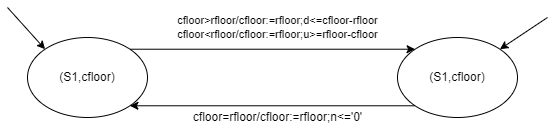
\includegraphics[width=1.2\textwidth]{3_1_elevator.png}
            \caption{题1流程图}
        \end{figure}

    \newpage

    \item[(2)]南北东西两个方向交通路口交通灯正交控制系统:南北方向直行绿灯40秒,东西方向直行绿灯30秒,黄灯5秒,在直行时可以左转,右转始终是自由的。正交控制系统是指南北方向为绿灯时东西方向为红灯,南北方向为红灯时东西方向为绿灯。为了满足安全以及提高通行要求,规定交通灯转换顺序为黄灯-->绿灯-->红灯-->黄灯。
    
    简要说明:
    \begin{enumerate}
        \item[(1)]考虑到实际情况安全问题,设置两向初态均为红灯; 
        \item[(2)]为实现该红绿灯正交系统,东西向红灯初始状态为10秒,南北向初始状态为45秒,如此可以保证当东西向为绿灯时,南北向刚好为红灯,对南北向同理.
        \item[(3)]理想系统中不会存在两灯同时绿灯的情况,但为避免外部环境所造成的偶然误差,在状态转移中增加了单绿灯设置,即当有一个灯为绿灯时,另外一个灯将阻塞为黄灯,直到另外一个灯转为红灯为止.
        \item[(4)]符号说明:  \par
        timeH:东西向红绿灯时间,\par
        timeV:南北向红绿灯时间,\par
        LightH:东西向红绿灯输出,\par
        LightV:南北向红绿灯输出,\par
    \end{enumerate}
   
        对该问题进行形式化建模:
        \begin{itemize}
            \item 状态集$S=\{S1\}$
            \item 初始状态$\{timeH=10,timeV=45,LightH=Red,LightV=Red\}$
            \item 数据变量集$X:\{timeH,timeV\}$
            \item 数据输入集$I_d:\{  \left[ 0,45 \right]  \}$
            \item 数据输出集$O_d:\{timeH,timeV\}$
            \item 控制输入集$I_c:\{\}$
            \item 控制输出集$O_c:\{LightH,LightV\}$ 
            \item 控制输出值集$:\{Red,Yellow,Green\}$ 
            
        \end{itemize}        
        转移条件和输出函数如图所示;
        \begin{figure}[!h]
            \centering
            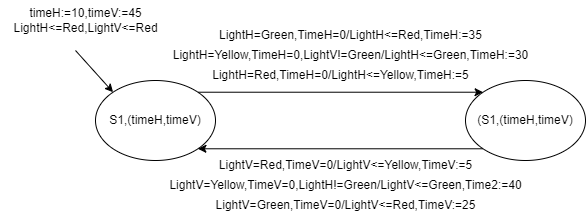
\includegraphics[width=1.2\textwidth]{3_2_Light.png}
            \caption{题2流程图}
        \end{figure}

    
    \item[(3)] 饮料售货机可以售3种饮料:可乐、茶和水。每瓶可乐售4元、每瓶茶售3元、每瓶水售2元;线上 (微信或支付宝)支付。每次可以购买1-3瓶饮料。

    符号说明:\par
    item:应为水、可乐、茶中的一个 \par
    number:选择个数,根据题意应不超过三个\par
    money:付款金额\par
    paytype:微信或支付宝 \par

    对该问题进行形式化建模:
    \begin{itemize}
        \item 状态集$S=\{S_{Init},S_{NumberSelect},S_{WaitPay}\}$
        \item 数据变量集$X:\{item,number,money,paytype\}$
        \item 初始状态:\{无,0,0,无\}
        \item 初始状态$\{d\}$
        \item 数据输入集$I_d$:\{无,水,可乐,茶,[0个,3个],[0元,12元],无,微信,支付宝\}
        \item 数据输出集$O_d:\{drink\}$
        \item 数据输出值集:\{水,可乐,茶\}
        \item 控制输入集$I_c:\{\}$
        \item 控制输出集$O_c:\{output\}$ 
        \item 控制输出值集$:\{Close,Open\}$ 
        
    \end{itemize}   
           
    转移条件和输出函数如图所示;

    \begin{figure}[!h]
        \centering
        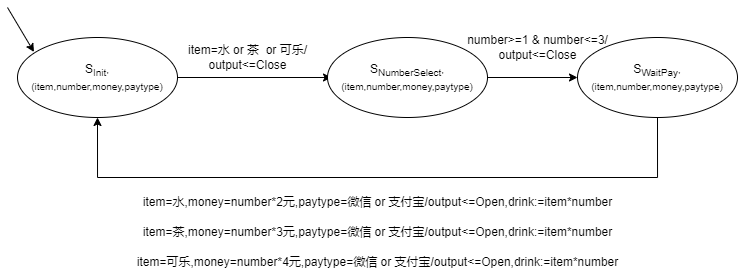
\includegraphics[width=1.2\textwidth]{3_3_Shopping.png}
        \caption{题3流程图}
    \end{figure}

\end{enumerate}
\end{document}